\chapter{Pondération du modèle}

\par Il existe deux niveaux de pondération dans le modèle: un premier, local, à l'intérieur de certains critères (champ de vision et champ de regard), et un deuxième, global, qui donne un poids à chacun des critères les uns par rapport aux autres. On a déjà abordé la pondération locale et ses hypothèses, on s'intéresse ici au second niveau de pondération: au global.

\par La pondération complète du modèle est un travail conséquent qui nécessite un engagement entier. On ne prétend donc pas donner la solution mais simplement des propositions pour une première approche théorique.

\section{Contraste, luminance, taille et champs visuels}
\par Comme on a pu voir dans les chapitres précédents, la construction du modèle se base sur la vision et sa modélisation. Une première piste importante pour la pondération peut être relevée à l'étude du modèle de Rose \citep{rose_sensitivity_1948}, qui, on le rappelle, est décrit par une simple équation (Eq. \ref{eq:modèle_rose_2}):

\begin{equation}
	BC^2\alpha^2 = \text{constant}
	\label{eq:modèle_rose_2} 
\end{equation}

\par On voit clairement qu'une importance supérieure est attribuée aux critères de contraste et de taille par rapport au critère de luminance avec des puissances d'ordre 2 par rapport à une puissance d'ordre 1. On peut donc dire que le contraste et la taille de l'objet nécessite une pondération (plus) forte. Si on ne peut pas relier directement la taille de l'objet perçu à l'acuité visuelle, il est important de noter que plus l'acuité est forte, plus l'objet sera perçu finement. Enfin, par expérience, il nous semble même que le contraste est un critère capital et qu'il devrait recevoir la plus forte des pondérations.

\par La pondération (locale et globale) des champs de vision et de regard est fortement liée à l'application qui est faite dans le système immersif. On a pu le constater via une expérimentation qui sera décrite dans le chapitre suivant.

\begin{table}[h]	
	\centering
	\caption{Force relative des critères du modèle non liés à la perception de la profondeur}
	\label{tab:ponderation_non_profondeur}
	\small
	\begin{tabular}{lc}
		\multicolumn{1}{l}{\bfseries Paramètre} & \multicolumn{1}{c}{\bfseries Force relative}\\		
		Contraste & Fort\\
		Taille de l'objet & Fort\\
		Champ de vision & Variable\\
		Champ de regard & Variable\\
		Luminance & Faible\\
	\end{tabular}
\end{table}

\section{Tracking, stéréoscopie, convergence des caméras et couleurs}
\par Une autre piste très intéressante est issue de l'importance relative des indices de profondeur entre eux. On a déjà présenté les différents indices qui permettent au cerveau de reconstruire une carte de profondeur (\textit{cf.} première partie sur l'état de l'Art). On s'intéresse ici à un classement par importance de ces indices.

\par Il existe quelques études qui ont comparé des indices de profondeurs entre eux afin de déterminer le(s)quel(s) est/sont prépondérant(s) sur les autres. Par exemple, \citep{mazur_relative_1990} compare la stéréoscopie avec la perspective aérienne et la comparaison de taille entre des objets familiers. \citep{reinhart_comparison_1990} ont comparé la taille relative des objets entre eux, la stéréoscopie (disparités binoculaires), l'interposition et la luminosité de l'objet, tandis que \citep{surdick_relevant_1994, surdick_perception_1997} comparent quant à eux 7 indices différents:

\begin{itemize}
	\item la luminance relative,
	\item la taille relative,
	\item la hauteur relative,
	\item la perspective linéaire,
	\item l'effet de rapprochement,
	\item le gradient de texture,
	\item la stéréoscopie.
\end{itemize}

\par Les résultats de \cite{mazur_relative_1990} et de \cite{surdick_relevant_1994} montrent une domination des indices de profondeur que sont la stéréoscopie et les perspectives aérienne et linéaire. Les résultats de \cite{reinhart_comparison_1990} mettent en avant l'apport de la stéréoscopie par rapport aux indices monoculaires pour la perception de la profondeur de manière plus tranchée. On note néanmoins que la grande majorité des indices mis en concurrence sont des indices graphiques qui sont donc en dehors de notre cadre d'étude.

\par Parallèlement, \citep{mikkola_relative_2010} relèvent que la stéréoscopie et la parallaxe de mouvement sont considérées comme les indices les plus importants (résultats à rapprocher de ceux de \citep{rogers_motion_1979} qui montrent que la parallaxe de mouvement est un indice de profondeur pertinent même lorsque tous les autres indices sont inexistants). Ils ont de leur côté conduit des expérimentations dans lesquelles ils demandaient à leurs sujets de noter de manière subjective l'impression de profondeur ressentie: la stéréoscopie arrive encore une fois avec de bon résultats tandis que des indices monoculaires tels que les ombres ou les textures des objets semblent avoir un impact plus réduit. Ces 

\par Enfin, \citep{mehrabi_making_2013} ont réalisé d'excellentes classifications sur les indices de profondeur, leurs atouts et leurs limitations (on trouvera une adaptation en Table \ref{tab:ponderation_depth_cues}) ainsi qu'une table sur les différentes techniques d'affichage en spécifiant notamment les indices de profondeurs disponibles dans chacun des cas. La classification est divisée en deux parties avec des indices ayant une contribution soit fort soit faible mais permet déjà une bonne approximation pour un idée générale de pondération.

\begin{table}[h]	
	\centering
	\caption{Force relative des indices de perception de la profondeur. Table adaptée depuis \citep{mehrabi_making_2013}}
	\label{tab:ponderation_depth_cues}
	\small
	\begin{tabular}{lccc}
		\multicolumn{1}{c}{\bfseries Indice de profondeur} & \multicolumn{1}{c}{\bfseries Indice binoculaire} & \multicolumn{1}{c}{\bfseries Force relative} & \multicolumn{1}{c}{\bfseries Portée}\\		
		Parallaxe binoculaire & Oui & Fort & $2,5~m - 20~m$\\
		Parallaxe monoculaire & Non & Fort & $0 - \infty$\\
		Taille de l'image rétinienne & Non & Fort & $0 - \infty$\\
		Perspective linéaire & Non & Fort & $0 - \infty$\\
		Gradient de texture & Non & Fort & $0 - \infty$\\
		Recouvrement & Non & Fort & $0 - \infty$\\
		Accommodation & Non & Faible & $0 - 2~m$\\
		Convergence & Oui & Faible & $0 - 10~m$\\
		Perspective aérienne & Non & Faible & \textit{Long. dist. seulement}\\
		Ombrage & Non & Faible & $0 - \infty$\\
		Couleurs & Non & Faible & $0 - \infty$\\
	\end{tabular}
\end{table}

\section{Conclusion}
\par Il reste néanmoins des critères pour lesquels la littérature ne donne pas immédiatement un a priori de pondération tels que le nombre d'images par seconde, la latence ou l'uniformité entre les écrans. par défaut on leur attribue une importance relative plus faible que les facteurs <<~forts~>> qui semblent très prépondérants sur les autres.

\par On a maintenant une meilleure idée générale des tendances qu'il peut exister pour une pondération du modèle dans le cas général. Dans des cas spécifiques (\textit{cf.} chapitre suivant) comme la conduite, la pondération peut fortement varier en fonction des besoins de l'utilisateur. On présente ces ordres de grandeur en Fig. \ref{fig:modèle_définitif_pondere} en modélisant les pondérations <<~fortes~>> avec une boite plus grande que les pondérations <<~faibles~>>.

\par Il convient de rappeler que cette proposition est une ébauche et que la définition précise d'une (ou de plusieurs) pondération(s) reste un sujet à part entière que nous n'avons pas à proprement parler traité.

\begin{figure}
	\centering
	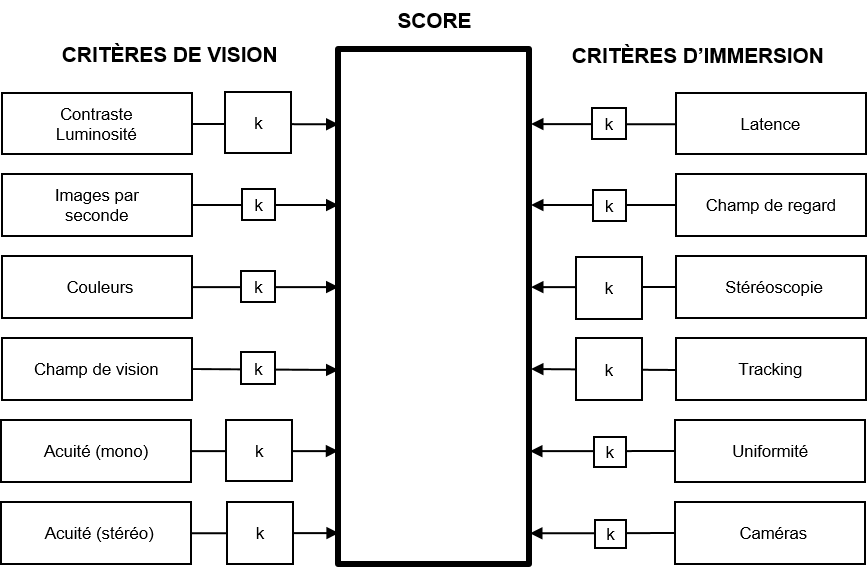
\includegraphics[scale=1]{Figures/ModeleDefinitifPondere}
	\caption{Modélisation avec ordre de grandeur de la pondération.}
	\label{fig:modèle_définitif_pondere}
\end{figure}